\chapter{Extending Geodesic DGGSs to Create 3D Prismatoid Grids} \label{chap:extension}
\cite{sirdeshmukh2019utilizing}
\cite{xie2013interactive}


\section{Prismatoid Grid Generation and Refinement}
Using the input DGGS as an input specification, our goal is to define the key elements of the corresponding 3D DGGS logically and consistently.
In this section, we discuss the approach for generating the initial discretization and define two refinement methods.


\subsection{Initial 3D Discretization} \label{sec:grid:discretization}
The initial 3D discretization is generated from the input polyhedron by extruding each face to cover the desired radial extent of the grid.
Faces are extruded outward to the desired maximum altitude, $R_\mathrm{max}$, and inwards to the desired minimum altitude, $R_\mathrm{min}$ (Figure~\ref{fig:abstract} top right).
These values become the maximum and minimum supported radii of the 3D DGGS, respectively.
If the minimum radius is zero, these base cells are pyramids; otherwise, they are frusta.
In both cases, the cells belong to a parent class of polyhedra known as prismatoids.
With this discretization, each cell represents the full radial domain of the grid; subsequent refinements will address this issue.


\subsection{Regular Prismatoid Refinement} \label{sec:grid:regular}
With an initial 3D discretization for the space of the grid system, we now need a method for refining cells to create more fine discretizations.
We also want to ensure that the 3D DGGS will make use of the same refinement scheme used by the input DGGS, referred to as the surface refinement.
For simplicity, we initially assume the surface refinement factor is 1:4; a generalization to other refinement factors is given in Section~\ref{sec:grid:factors}.


\begin{figure}[h]
	\centering
	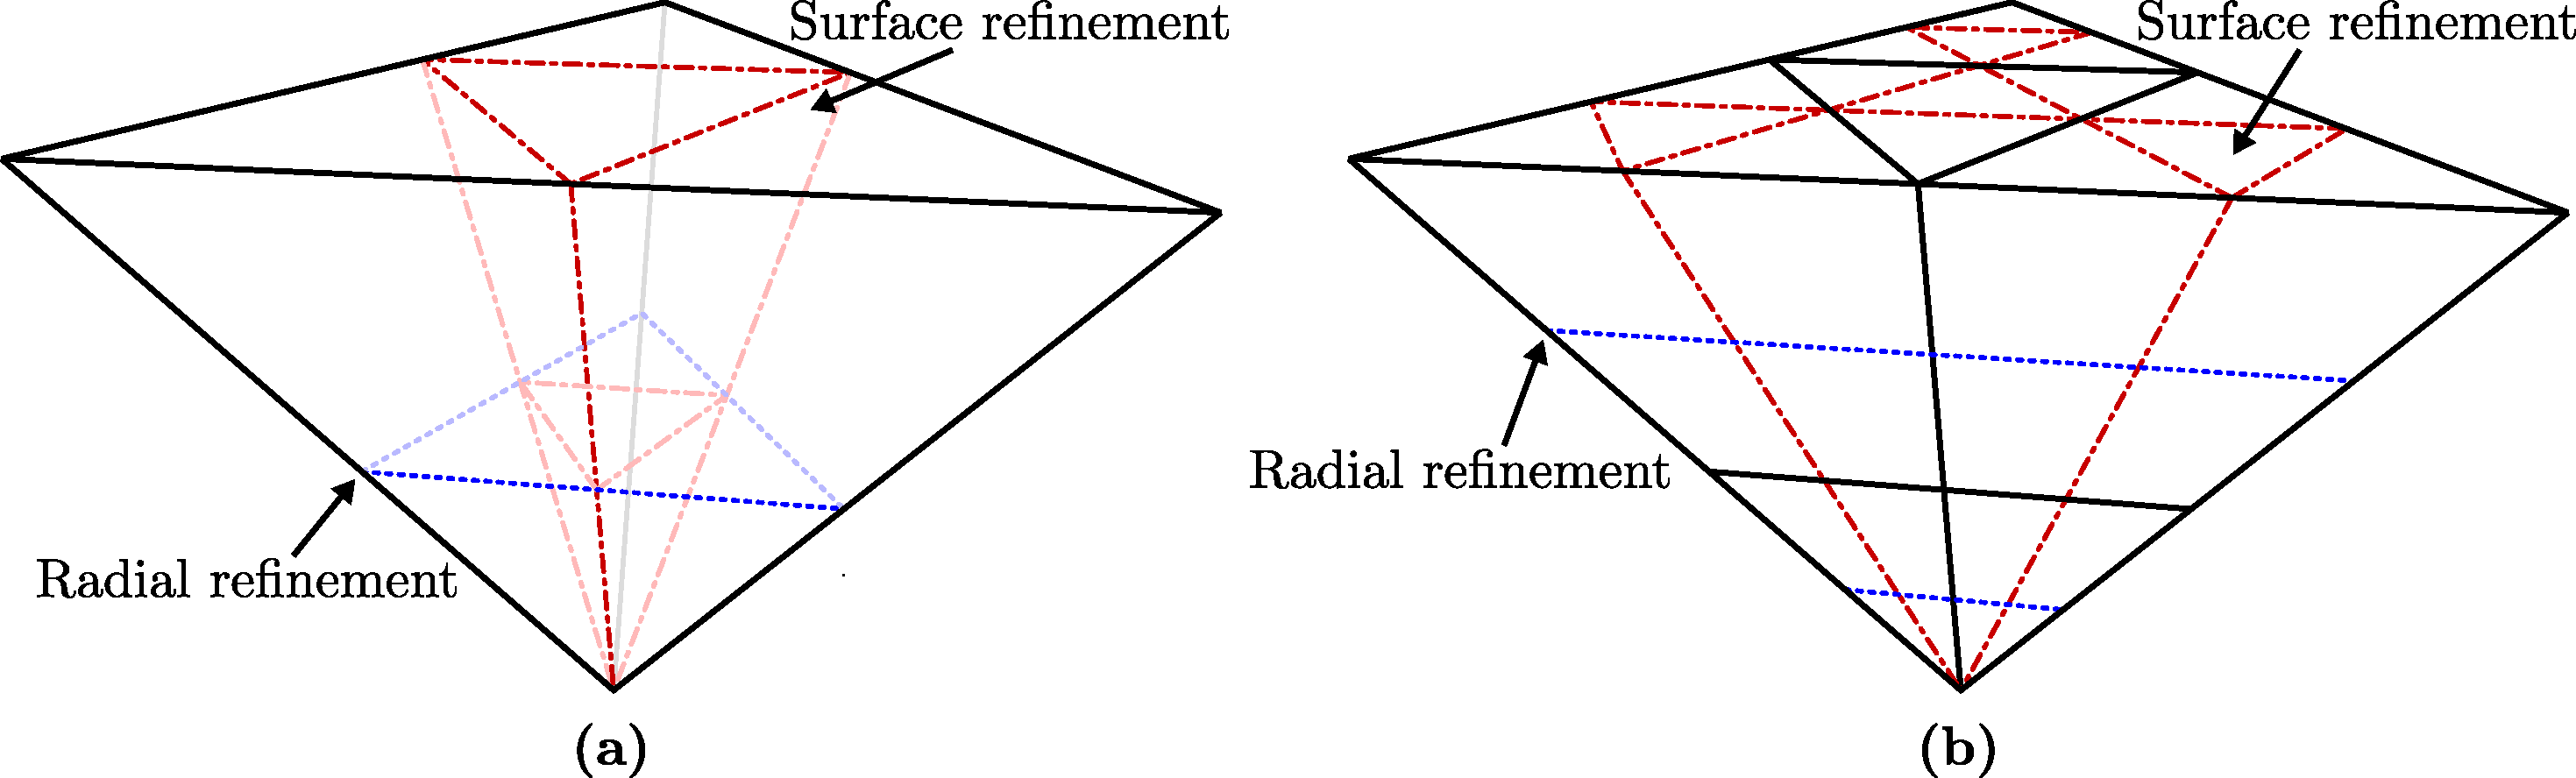
\includegraphics[width=\columnwidth]{reg-refinement.pdf}
	\caption{Regular prismatoid refinement as applied to a single pyramid cell \textbf{(a)} once and \textbf{(b)} twice}
	\label{fig:regular}
\end{figure}


The regular method for refining prismatoid cells is shown in Figure~\ref{fig:regular}.
The bases of the cells are refined using the surface refinement and the resulting edges extruded to meet.
At the same time, a radial split is placed at the midpoint between the two bases.
This refinement results in an inner and outer layer of cells, each containing the same number of cells as one another.
The outer layer is always composed of frustum cells, whereas the inner layer has the same shape as the cells that were being refined.
This refinement can then be repeated, treating each of the new layers the same as the initial discretization.
Defining the refinement in terms of layers of cells as opposed to individual cells allows non-congruent surface refinements to be accommodated inherently.


\subsection{Semiregular Prismatoid Refinement} \label{sec:grid:degen}
While the regular prismatoid refinement proposed above is simple, it has a key drawback if the ratio between $R_\mathrm{max}$ and $R_\mathrm{min}$ is large.
In this situation, layers that are near the minimum radius end up being much smaller than those near the maximum.
A different refinement method is needed to generate more uniformly sized cells.
To do this, we classify the layers of the grid as either central or normal.
We use $r_\mathrm{min}$ and $r_\mathrm{max}$ to refer to the minimum and maximum radius of a layer, respectively.
Central layers are those that border the innermost portion of the grid ($r_\mathrm{min} = R_\mathrm{min}$) and all other layers are considered normal.
By definition, at any resolution of the 3D DGGS, there is only one central layer.
Furthermore, the initial discretization is entirely composed of this central layer.
We continue our assumption of a 1:4 surface refinement factor from before.


\begin{figure}[h]
	\centering
	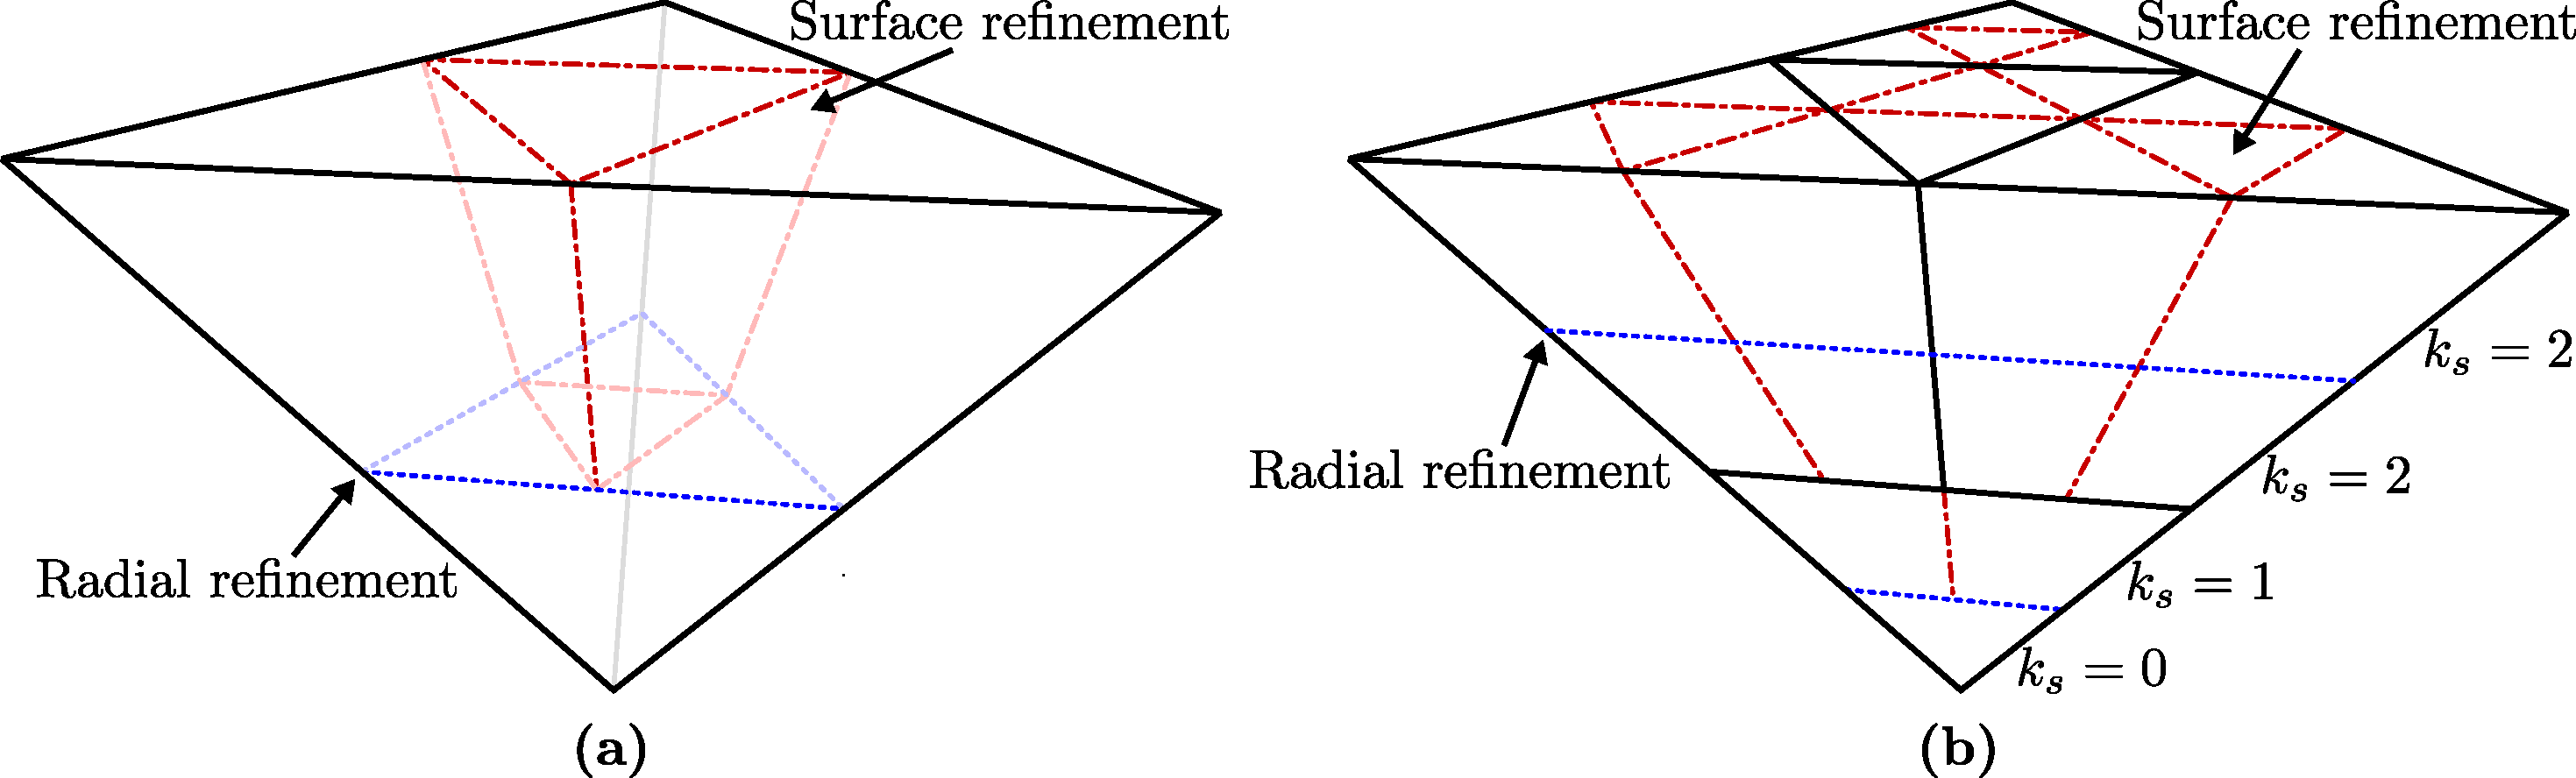
\includegraphics[width=\columnwidth]{semireg-refinement.pdf}
	\caption{Semiregular prismatoid refinement as applied to a single pyramid cell \textbf{(a)} once and \textbf{(b)} twice.
		In \textbf{(b)}, the number of times the surface refinement has been applied ($k_s$) is shown for each layer; see how the radial refinements of central layers separate regions of the grid with different values of $k_s$}
	\label{fig:semiregular}
\end{figure}


In this refinement scheme, refinement of central layers is different from the above regular method.
We assert that $R_\mathrm{min}$ be treated as equal to zero, and therefore central layers are composed of pyramid cells.
If the actual value of $R_\mathrm{min}$ is not zero, then any resulting layers below this radius can be discarded or ignored.
Just as before, the bases of the pyramid cells are refined using the surface scheme, and a radial split is made in the middle of the layer.
However, the new edges do not extend fully toward the apex of the pyramid but instead are stopped at the radial split (Figure \ref{fig:semiregular}).
This refinement results in two new layers: an inner central layer, which is similar to the initial central layer, and an outer normal layer.
As demonstrated in Figure~\ref{fig:semiregular}b, the resolution---or refinement level---a layer appears in at the 3D grid does not necessarily correspond to how many times the surface refinement scheme has been applied to it.
We define the number of times the surface refinement has been applied to a given layer as the surface resolution, given by $k_s$.
Thus, if we say the initial discretization has $k_s = 0$, after one level of refinement the inner central layer also has $k_s = 0$, whereas the normal layer has $k_s = 1$.
This surface resolution is needed for grid encoding/decoding and various indexing queries, but as will be seen later can be computed and does not need to be explicitly stored.


\begin{figure}[h]
	\centering
	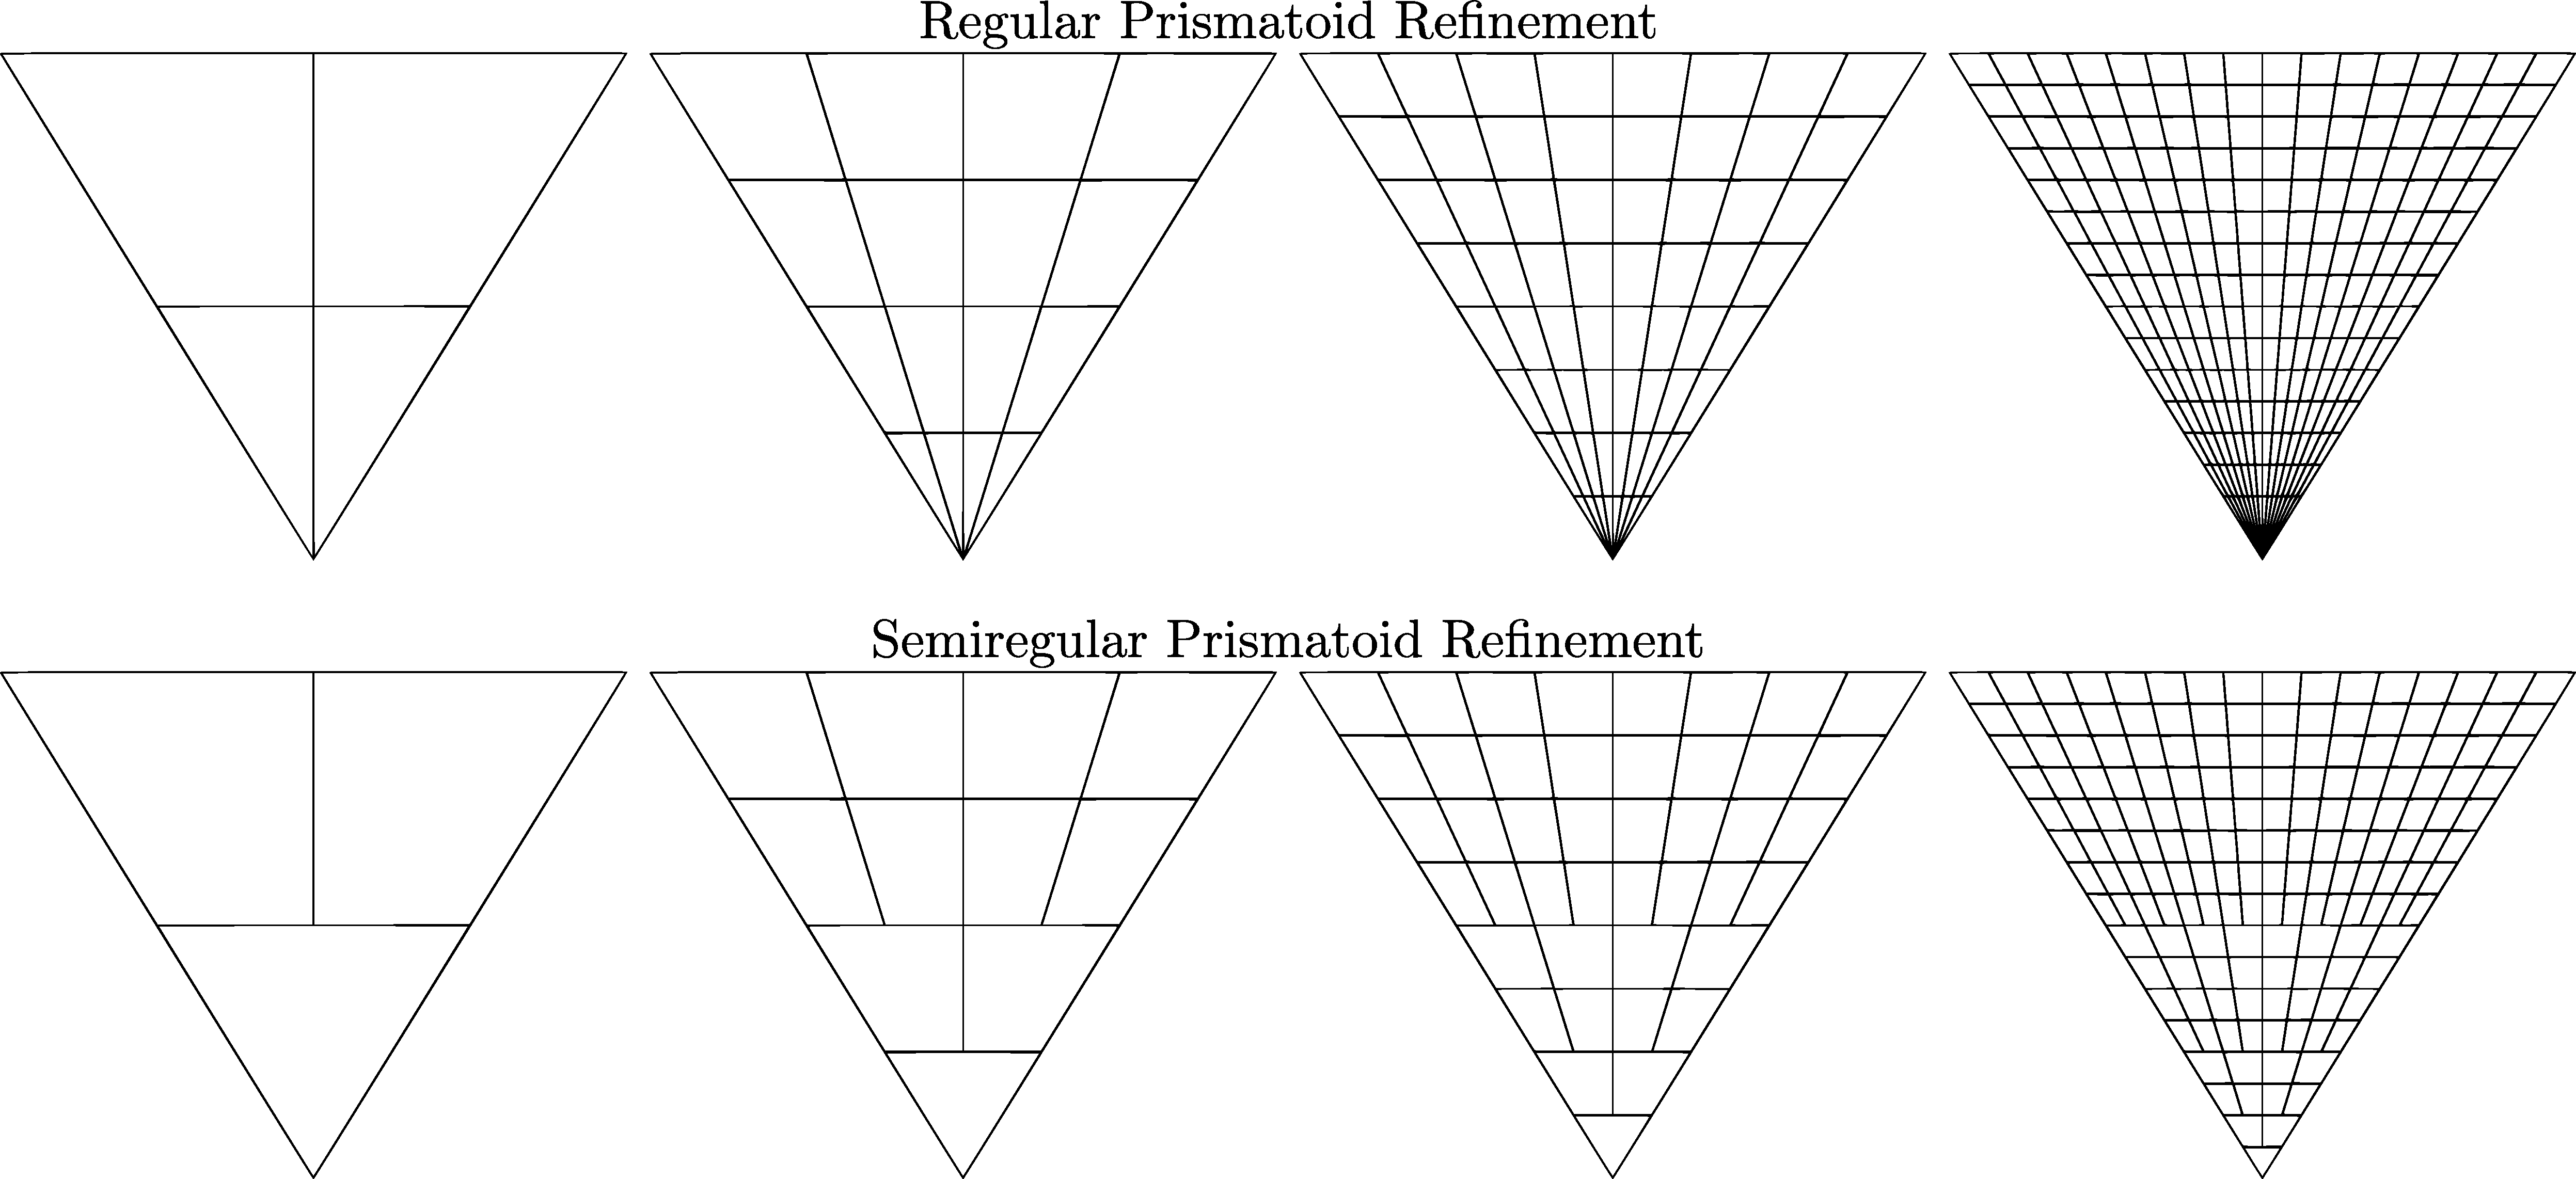
\includegraphics[width=\textwidth]{reg-vs-semireg.pdf}
	\caption{Three levels of successive applications of regular (top) and semiregular (bottom) prismatoid refinement.
		Only the side of a single pyramid starting cell is shown to highlight the behaviour of the two schemes at different radii.
		Note how cells degenerate towards the centre with regular refinement, whereas this issue is not present in the semiregular scheme}
	\label{fig:regVsemireg}
\end{figure}


Normal layers in this scheme are simply refined using regular prismatoid refinement.
This results in two normal layers, both of which have $k_s$ equal to one greater than that of the starting layer.
Figure~\ref{fig:regVsemireg} compares three successive applications of regular and semiregular prismatoid refinement to a single pyramid cell.

\section{Refinement Extensions}
\subsection{Other Surface Refinement Factors} \label{sec:grid:factors}
While it is possible to use the above refinement methods for surface refinement factors other than 1:4, doing so results in a potentially significant issue that should be addressed.
To address this challenge, we introduce the idea of a one-dimensional (1D) refinement factor.
We can find the 1D refinement factor by taking the square root of the surface (2D) one.
For example, the 1D refinement factor of a 1:4 surface refinement scheme (Figures~\ref{fig:regular} and \ref{fig:semiregular}) is 1:2.
While the surface refinement scheme need not be uniform across the two dimensions, the 1D refinement factor gives an idea of the \textit{average} refinement that is expected along each dimension.


To create uniform cells, it is clear that the refinement factor along the radial dimension for regular prismatoid refinement should be equal to the 1D refinement factor.
If this is not the case, then the width of cells relative to their depth is not constant between refinement levels, since one dimension is refined more quickly.
For a surface refinement factor of 1:4, the single radial split used matches this exactly (one split creates two new layers).
For other surface refinement factors, the 1D and radial refinement factors are not necessarily equal, and cell shape will degenerate---becoming either increasingly narrow or wide---as refinement continues.


To address this issue, we modify the number of radial splits performed such that the number of layers produced is equal to the 1D refinement factor.
For surface refinement factors that are perfect squares (e.g.
1:4, 1:9) this is trivial, as the 1D refinement factor is an integer; the corresponding radial refinement factor is achieved by creating a number of layers equal to the 1D factor.
For other surface refinement factors, though, this becomes more difficult.
The 1D refinement factor is no longer an integer, and since we can only perform a whole number of radial splits, the 1D and radial refinement factors cannot be exactly equal.
To address this issue, we propose performing a different number of radial splits at different levels of refinement to make the average radial refinement factor equal to the 1D one.


There are a few different methods that can be used to determine the number of radial splits to perform at a given refinement level.
The most simple method is to simply alternate between producing one layer (i.e.
no splits) and producing a number of layers equal to the surface refinement factor.
When the surface refinement factor is not a prime number, a better method is to alternate between the two members of a factor pair, such as two and three for a 1:6 surface factor.
In general, the product of the number of layers at each level of refinement should be equal to (or as close as possible to) the 1D refinement factor to the power of the number of refinement levels.
Formally,

\begin{equation*}
\prod_{i = 1}^{k} \ell_{i} = f^{k},
\end{equation*}
%
where $\ell_{i}$ is the number of layers produced at refinement level $i$, $k$ is the level of refinement, and $f$ is the 1D refinement factor.
This equation can be used iteratively to find the best number of layers for successive levels of refinement for prime surface refinement factors.
Table~\ref{tab:layers} lists our proposed layering sequences for surface refinement factors from 1:2 up to 1:9.


\begin{table}[h]
	\centering
	\begin{tabular}{@{}cl@{}}
		\toprule
		Surface Refinement Factor & Layering Sequence       \\ \midrule
		1:2                  & \textbf{2,1,2,1}             \\ 
		1:3                  & \textbf{3,1,3,1}             \\ 
		1:4                  & \textbf{2,2,2,2}             \\ 
		1:5                  & 2,3,2,2,2,3,2,2,2,3,2,2,3... \\ 
		1:6                  & \textbf{3,2,3,2}             \\ 
		1:7                  & 3,2,3,3,2,3,3,2,3,3,3,2,3... \\ 
		1:8                  & \textbf{4,2,4,2}             \\
		1:9                  & \textbf{3,3,3,3}             \\ \bottomrule
	\end{tabular}
	\caption{Our proposed layering sequences for different surface refinement factors.
		Each number in the sequence is how many layers \textit{normal} layers should split into at the corresponding level of refinement.
		Bold indicates that the sequence repeats indefinitely.
		For semiregular prismatoid refinement---since the initial discretization has no normal layers---these sequences are used starting with the \textit{second} level of refinement}
	\label{tab:layers}
\end{table}


\begin{figure}[h]
	\centering
	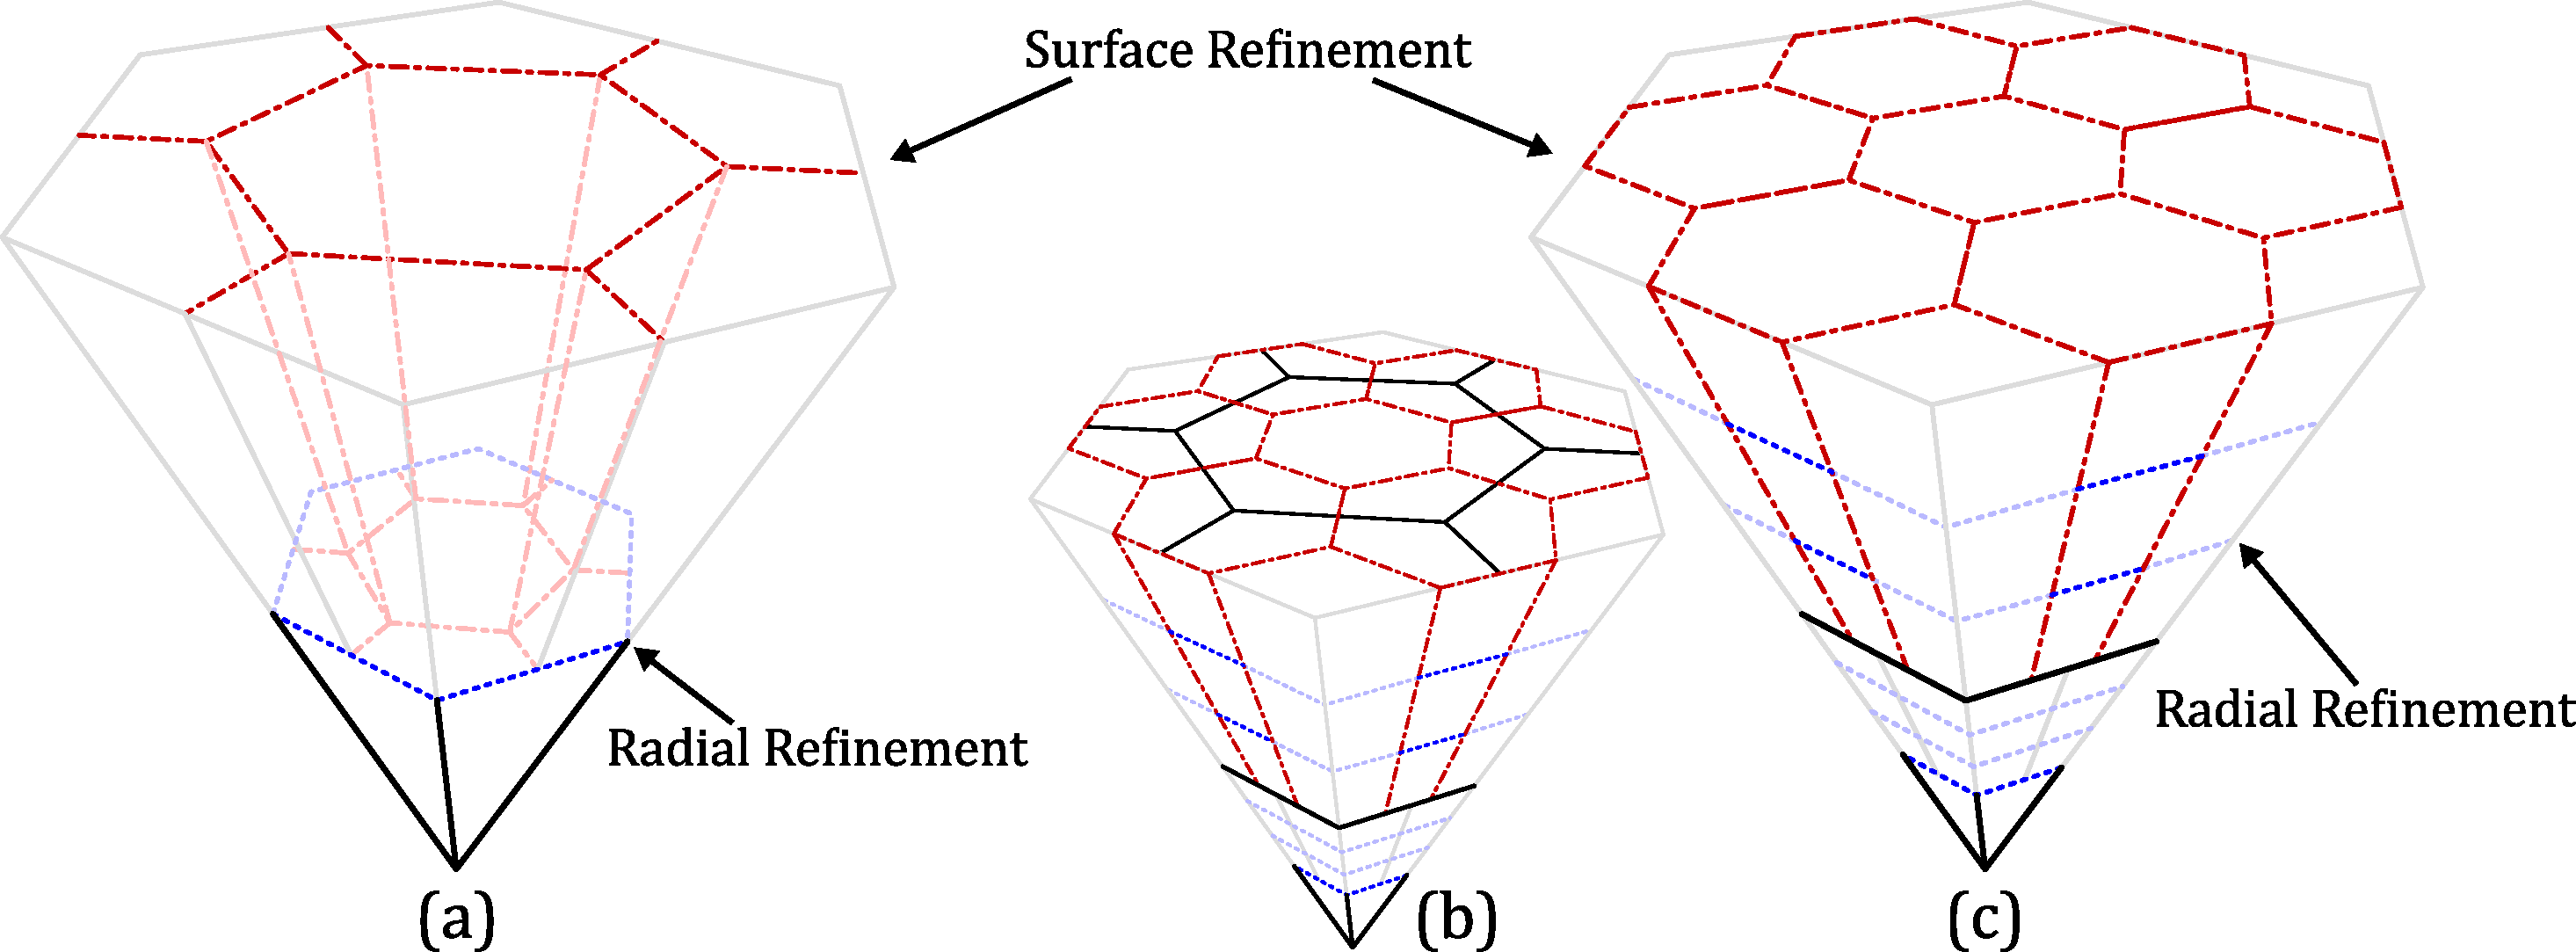
\includegraphics[width=\textwidth]{semireg-hexagons.pdf}
	\caption{Semiregular prismatoid refinement applied to a hexagonal base cell using a 1:3 surface refinement scheme \textbf{(a)} once and \textbf{(c)} twice; \textbf{(b)} is the same image as \textbf{(c)}, but with the surface cells of the previous refinement level shown for reference.
		Note that in the second level of refinement, normal layers have two radial refinements as opposed to one}
	\label{fig:hexagons}
\end{figure}


An example of semiregular prismatoid refinement with 1:3 hexagonal surface refinement is shown in Figure~\ref{fig:hexagons}.
The first level of refinement is identical to the cases for a 1:4 surface refinement factor since no normal layers have been refined.
In the second level, however, two radial splits are performed in the normal layers as opposed to one.
In the next level of refinement, which is not shown, normal layers would not have any radial refinements per the proposed sequence in Table~\ref{tab:layers}.


\subsection{Cell Aspect Ratio} \label{sec:grid:ar}
The surface and radial dimensions of Earth are inherently very different, and because of this, it is often desirable for these two dimensions to be at different resolutions in a 3D geospatial grid.
For our 3D DGGSs, achieving this entails changing the width of cells in the grid (surface resolution) relative to their depth (radial resolution).
We refer to the ratio between a cell's width and depth the \textit{aspect ratio} of the cell.
While the refinement methods described thus far do a good job of producing cells with a similar aspect ratio---both between cells in the same and different resolutions---there is no direct mechanism for controlling what this aspect ratio will be.
To address this issue, we introduce two modifications that can be made to prismatoid refinement to decrease and increase the aspect ratio.


In order to decrease the aspect ratio of cells in the grid, the number of times the surface refinement is applied relative to the number of radial splits should be increased.
Since further applications of the prismatoid refinement will maintain the expected cell aspect ratio (a result of the surface and expected radial refinement factors being equal), this only needs to be done the first time a layer would have the bases of its cells refined with the surface scheme.
Thus, for semiregular prismatoid refinement, this is done while refining the outer normal layer that results from refining central layers.
In the case where only regular prismatoid refinement is used, this is then only done during the first level of refinement.


Likewise, to increase the aspect ratio of cells, we need to decrease the number of times the surface refinement scheme is applied relative to the number of radial splits.
This is done by first \textit{not} applying the surface refinement to a layer the first time it would usually be done, and if needed applying additional radial splits at the same time.
These modifications would be done at the same time as the method for decreasing the aspect ratio for the same reasons.


Therefore, given some target cell aspect ratio $a$, we must determine which of the above methods to use.
To do this, we must first quantify the width and depth of a cell.
More specifically, we need to define the average width and depth of cells in a layer, since refinement is performed by layer and not by cell.
Depth comes trivially from the radial extent of the layer ($r_\mathrm{max} - r_\mathrm{min}$).
There are many potential ways to measure the width of a cell; for our purposes, we chose to use the square root of its area.
This choice ensures the framework will produce consistent results for input polyhedra with the same number of faces, irrespective of the shape(s) of said faces.


For the region of outer normal layer(s) generated by refining central layers, we can say the average depth of cells is the total depth of the region divided by the number of layers in the region (assuming no applications of the surface refinement scheme).
Let $\upsilon$ be the percentage of $r_\mathrm{max}$ occupied by this region and $x$ be the number of extra radial splits, then we have

\begin{equation*}
\frac{\upsilon r_\mathrm{max}}{x+1}.
\end{equation*}
%
Likewise, the average cell width in this region is the surface area of the sphere divided by the number of cells (assuming no extra radial splits).
Let $n$ be the number of faces on the input polyhedron and $w$ be the number of times the surface refinement is applied, then the number of cells is $n f^{2w}$ and the average cell width is

\begin{equation*}
\sqrt{ \frac{ 4 \pi r_\mathrm{max}^2 }{ n f^{2 w} } } = \frac{2 r_\mathrm{max}}{f^w} \sqrt\frac{\pi}{n}.
\end{equation*}
%
We can now equate these using the desired aspect ratio to solve for $x$ and $w$, giving

\begin{equation*}
a \frac{\upsilon}{x+1} = \frac{2}{f^w} \sqrt\frac{\pi}{n}.
\end{equation*}
%
As to not violate our prior assumptions, when solving for one variable the other is set to zero; this ensures only one of the two strategies for modifying the aspect ratio is employed.
Setting $w = 0$ we get

\begin{equation}
x = \frac{a \upsilon}{2} \sqrt{\frac{n}{\pi}} - 1,
\label{eq:extraSplits}
\end{equation}
%
and setting $x = 0$ we get

\begin{equation}
w = \log_{f} \left( \frac{2}{a \upsilon} \sqrt{ \frac{\pi}{n}} \right).
\label{eq:num2D}
\end{equation}


\begin{figure*}[h]
	\centering
	\begin{subfigure}[]{0.25\textwidth}
		\centering
		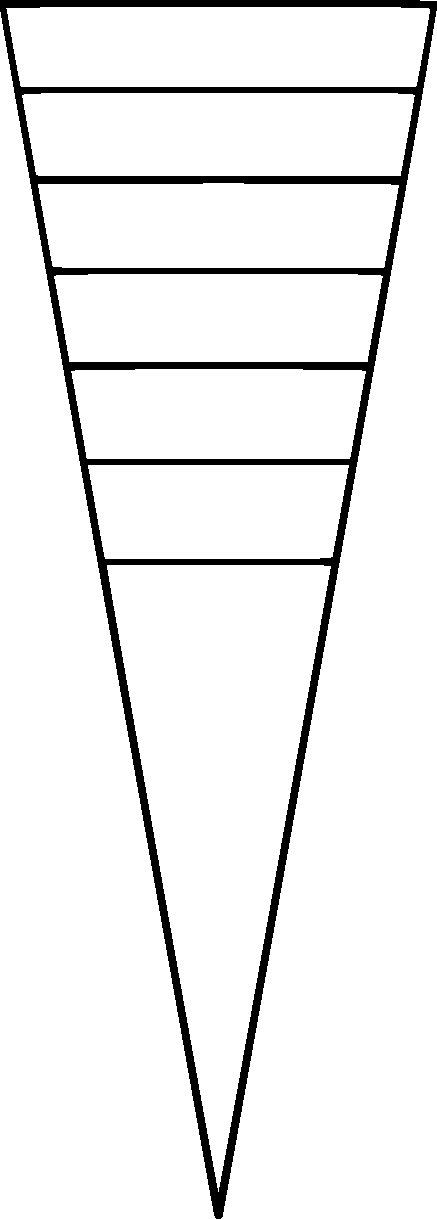
\includegraphics[width=0.5\columnwidth]{5-ers.pdf}
		\caption{}
		\label{fig:ers1}
	\end{subfigure}%
	%
	\begin{subfigure}[]{0.25\textwidth}
		\centering
		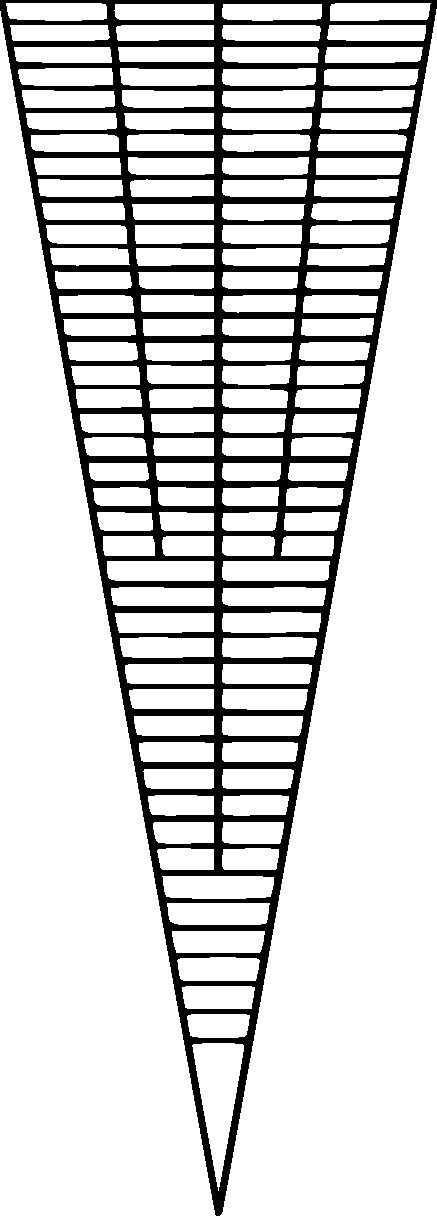
\includegraphics[width=0.5\columnwidth]{5-ers3.pdf}
		\caption{}
		\label{fig:ers3}
	\end{subfigure}%
	%
	\begin{subfigure}[]{0.25\textwidth}
		\centering
		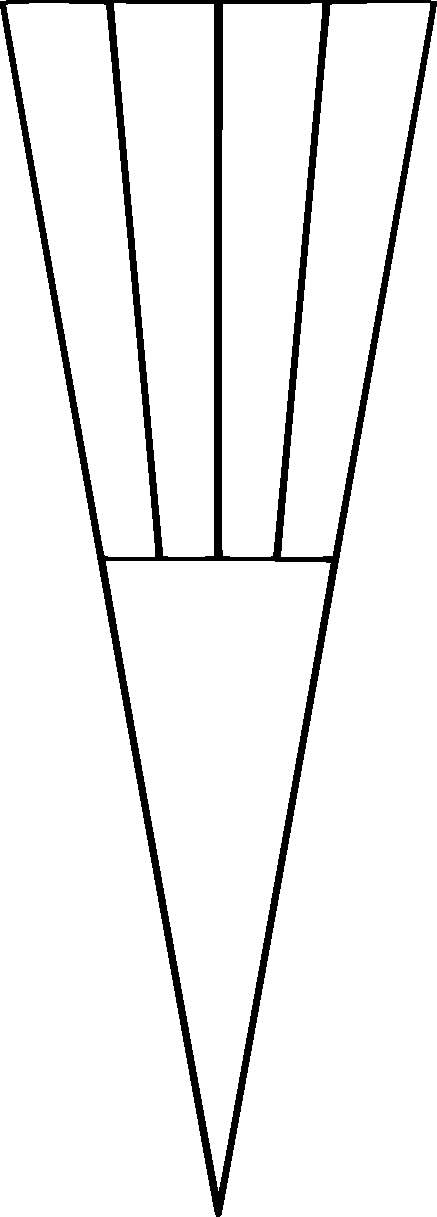
\includegraphics[width=0.5\columnwidth]{2-ess.pdf}
		\caption{}
		\label{fig:ess1}
	\end{subfigure}%
	%
	\begin{subfigure}[]{0.25\textwidth}
		\centering
		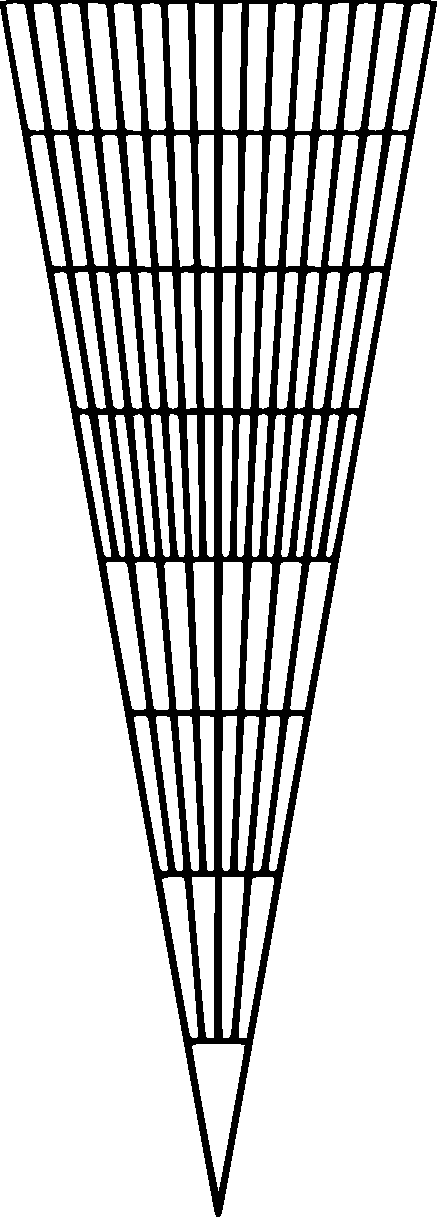
\includegraphics[width=0.5\columnwidth]{2-ess3.pdf}
		\caption{}
		\label{fig:ess3}
	\end{subfigure}
	
	\caption{A demonstration of how refinement can be modified to affect the aspect ratio of cells.
		All figures show a starting pyramid cell from a grid with 200 cells in its initial discretization.
		Central layer with five extra radial splits ($a = 3$ to get $x = 5$) at \textbf{(a)} one level of refinement and \textbf{(b)} three levels.
		Central layer with two applications of the surface refinement scheme ($a = 1/8$ to get $w = 2$) at \textbf{(c)} one level of refinement and \textbf{(d)} three levels}
	\label{fig:extraDPS}
\end{figure*}


The actual values of $x$ and $w$ selected for use is determined by which one is negative.
If $x$ is negative, it is set to zero, and the value of $w$ is used---vice versa for if $w$ is negative.
Since $x$ or $w$ may not be integers, we simply round them to the nearest whole number to get the actual value to be used during refinement.
The results of refinement with different target aspect ratios are demonstrated in Figure~\ref{fig:extraDPS}.

\section{Summary}